% !TeX spellcheck = en_US
%\documentclass{beamer}
\documentclass[handout]{beamer}
\usepackage[spanish]{babel}
\usepackage[utf8]{inputenc}
\usepackage{graphicx}
\usepackage{tcolorbox}
\usepackage{color}

\usepackage{braket}
\usepackage{hyperref}
%\setbeamercolor{frametitle}{fg=white}
%\usefonttheme{structuresmallcapsserif}
\setbeamertemplate{footline}[frame number]
\setbeamerfont{footnote}{size=\tiny}

\setbeamercolor{page number in head/foot}{fg=black}

\usepackage{amsmath}
\usepackage{mhchem}
\usepackage{tikz}
\def\checkmark{\tikz\fill[scale=0.4](0,.35) -- (.25,0) -- (1,.7) -- (.25,.15) -- cycle;} 

\usepackage{default}

\usepackage[backend = bibtex, style = verbose, sorting = none, autocite = footnote]{biblatex}
\addbibresource{references.bib}

\newcommand\blfootnote[1]
{%
	\begingroup
	\renewcommand\thefootnote{}\footnote{#1}%
	\addtocounter{footnote}{-1}%
	\endgroup
}
\newcommand{\fcite}[1]{\blfootnote{\cite{#1}}}

\usetheme{Berkeley}

\begin{document}
	\begin{frame}
		\centering
		%\color{white}
		\textsc{\large Photocatalytic and electrocatalytic reduction of \ce{CO2} to methanol by the homogeneous pyridine-based systems}
		\\
		\vspace{0.5cm}
		{\scriptsize Wai Wang, Junxiao Zhang, Hui Wang, Lianjia Chen, Zhaoyong Bian}
		\\
		\vspace{3cm}
		\raggedleft Juan Barbosa \\
		\raggedleft \small Catálisis en la industria y el laboratorio
	\end{frame}

\begin{frame}{Contenidos}
	\tableofcontents
\end{frame}

\section{Introducci\'on}
\begin{frame}{Introducci\'on}
	\begin{figure}[h]
		\centering
		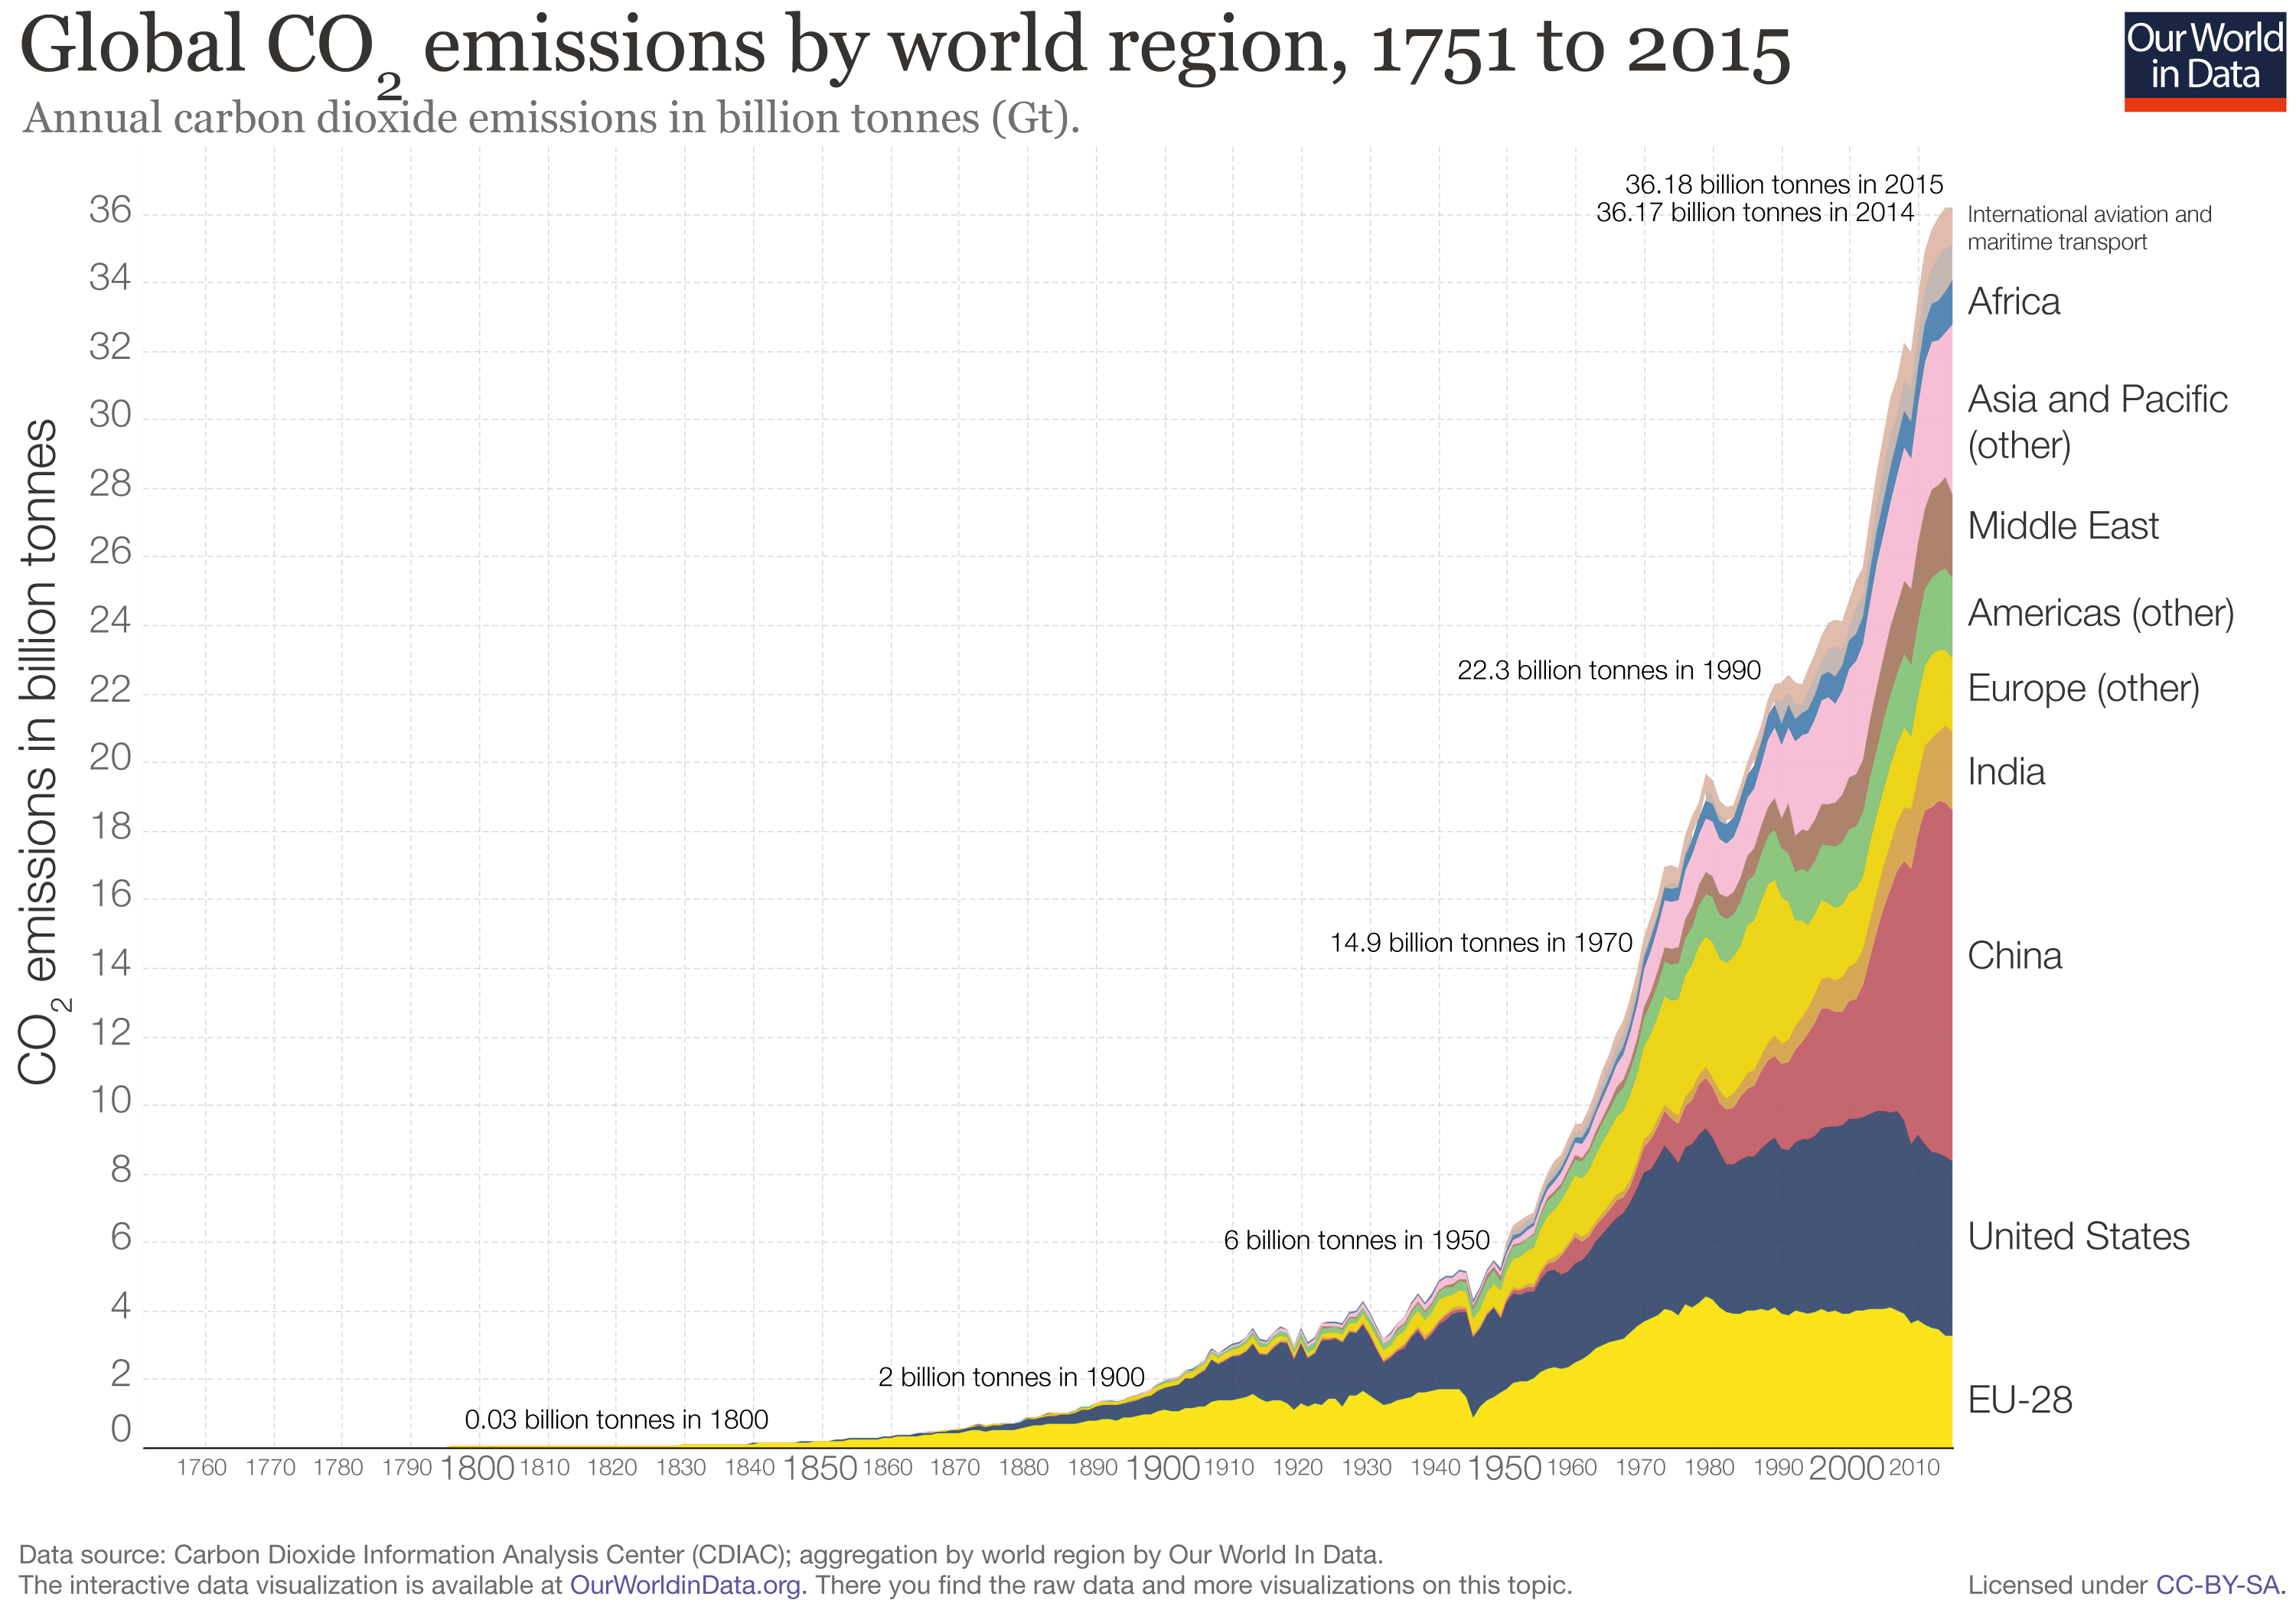
\includegraphics[width=\linewidth]{sources/CO2_emissions}
	\end{figure}
\end{frame}

\begin{frame}{Introducci\'on}
	\begin{itemize}
		\item La conversi\'on de \ce{CO2} a combustibles y energ\'ias renovables tiene efectos importantes en el medio ambiente y los sectores energ\'eticos.
		\item Dentro de estos procesos de conversi\'on se  encuentra la reducci\'on electroqu\'imica de \ce{CO2}.
		\begin{itemize}
			\item Permite obtener alquenos y alcoholes.
			\item Baja selectividad.
			\item No existe claridad sobre los mecan\'ismos.
			\item Aplicaci\'on de $V$ grandes, que inducen a altos consumos energ\'eticos.
		\end{itemize}
	\end{itemize}
\end{frame}

\begin{frame}{Introducci\'on}
	\begin{itemize}
		\item La reducci\'on fotocatal\'itica constituye una ruta atractiva, pues usa la abundancia de la radaci\'on solar para la utilizaci\'on del \ce{CO2}.
		\begin{itemize}
			\item \textbf{Fotoreducci\'on homog\'enea} usando un catalizador molecular.
			\item \textbf{Fotoreducci\'on heterog\'enea} usando semiconductores.
			\begin{itemize}
				\item \ce{TiO2} \ce{SiC} $\longrightarrow$ \ce{CO}, \ce{MeOH}, \ce{CH4}.
			\end{itemize} 
		\end{itemize}
	\end{itemize}
	\begin{figure}[h]
		\centering
		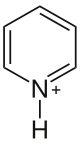
\includegraphics[width=0.1\linewidth]{sources/pyridinium}
	\end{figure}
	Ion piridinio logra hasta 30 \% de rendimiento Far\'adico para metanol en electrodos de paladio hidrogenados.
\end{frame}

\begin{frame}{Introducci\'on}
	\begin{figure}[h]
		\centering
		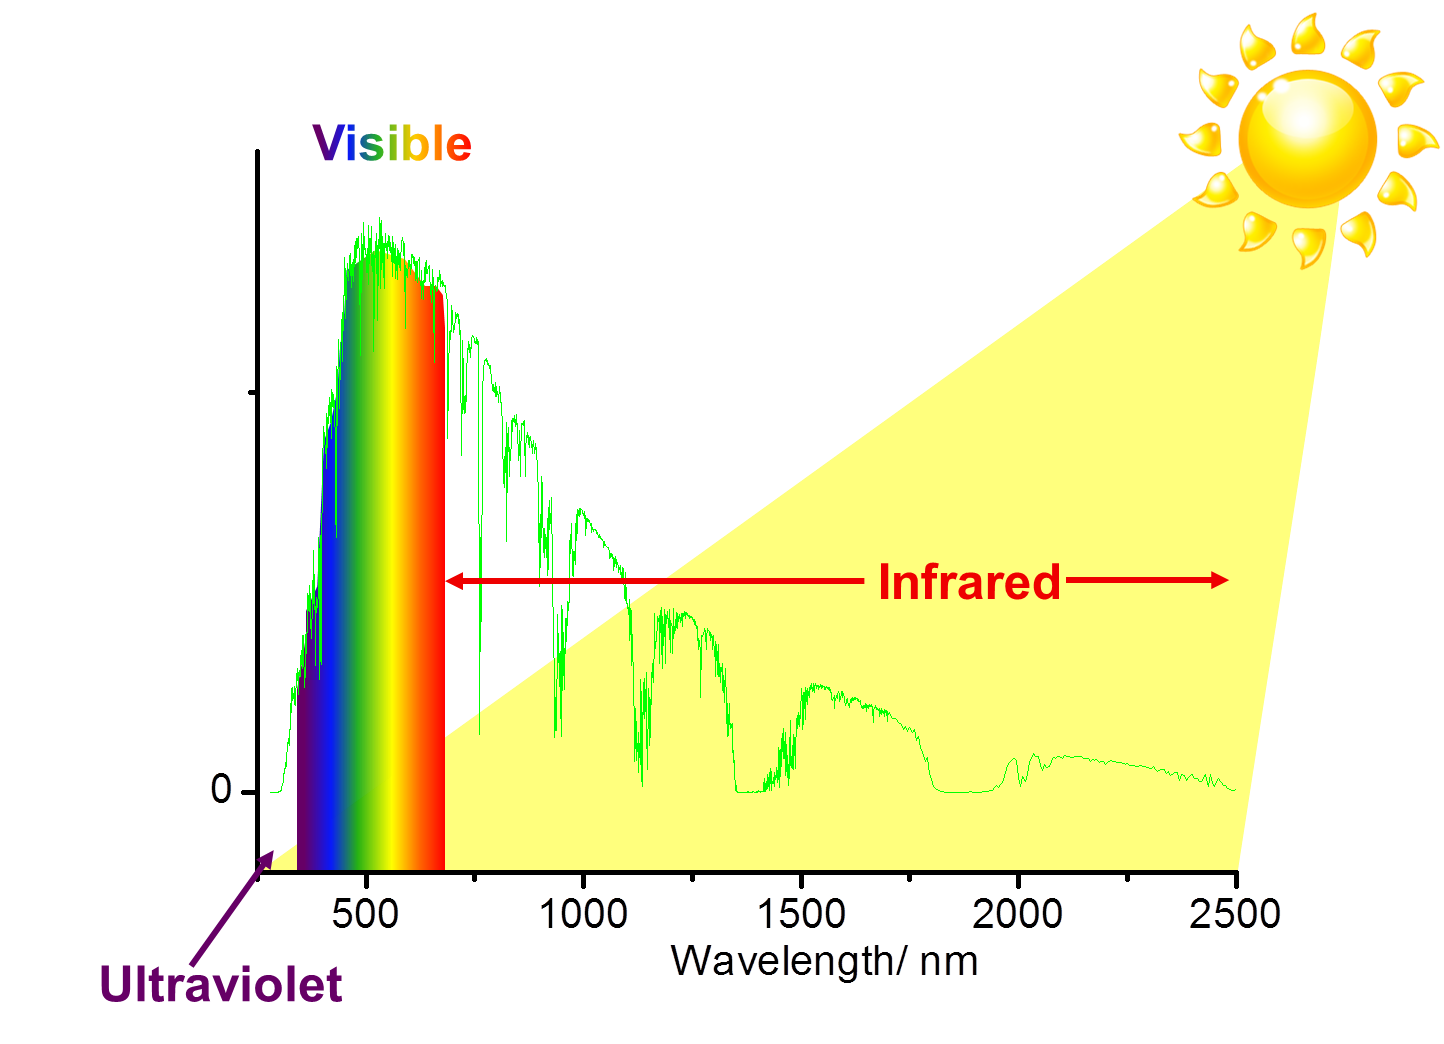
\includegraphics[width=0.8\linewidth]{sources/spectrum}
	\end{figure}
	\begin{itemize}
		\item Complejos de renio absorben mayormente en el UV.
		\item Bajo TON, y selectividad.
	\end{itemize}
\end{frame}

\section{Procedimiento experimental}
\begin{frame}{Procedimiento experimental}
	Preparaci\'on de \ce{[Ru(phen)_3](PF6)2}.
	\begin{itemize}
		\item Reflujo por 8 horas.
		\begin{equation*}
			\ce{EtOH}(l) + 
			\begin{cases}
				\ce{RuCl3} &  \text{(0.42 g, 2 mmol)} \\
				\ce{1,10-fenantrolina} & \text{(1.09 g, 6 mmol)}
			\end{cases}
			+ \ce{N2(g)}
		\end{equation*}
		\item Posteriormente se adiciona \ce{NH4PH6} (3.26 g, 20 mmol).
		\item El s\'olido se filtra y se seca al vac\'io.
	\end{itemize}
\end{frame}

\begin{frame}{Procedimiento experimental}
	\footnotesize
	\begin{columns}
		\begin{column}{0.2\linewidth}
			\textbf{$^1$HRMN}
			\begin{figure}[h]
				\centering
				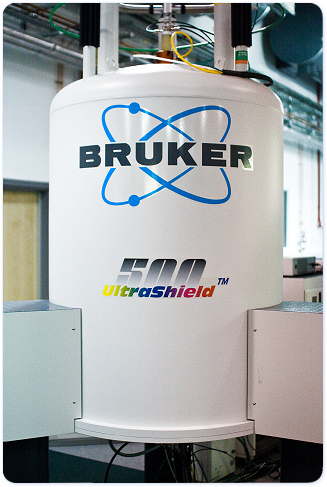
\includegraphics[width=\textwidth]{sources/bruker}
			\end{figure}
		\end{column}
		\begin{column}{0.25\linewidth}
			\textbf{Absorci\'on UV-vis}
			\begin{figure}[h]
				\centering
				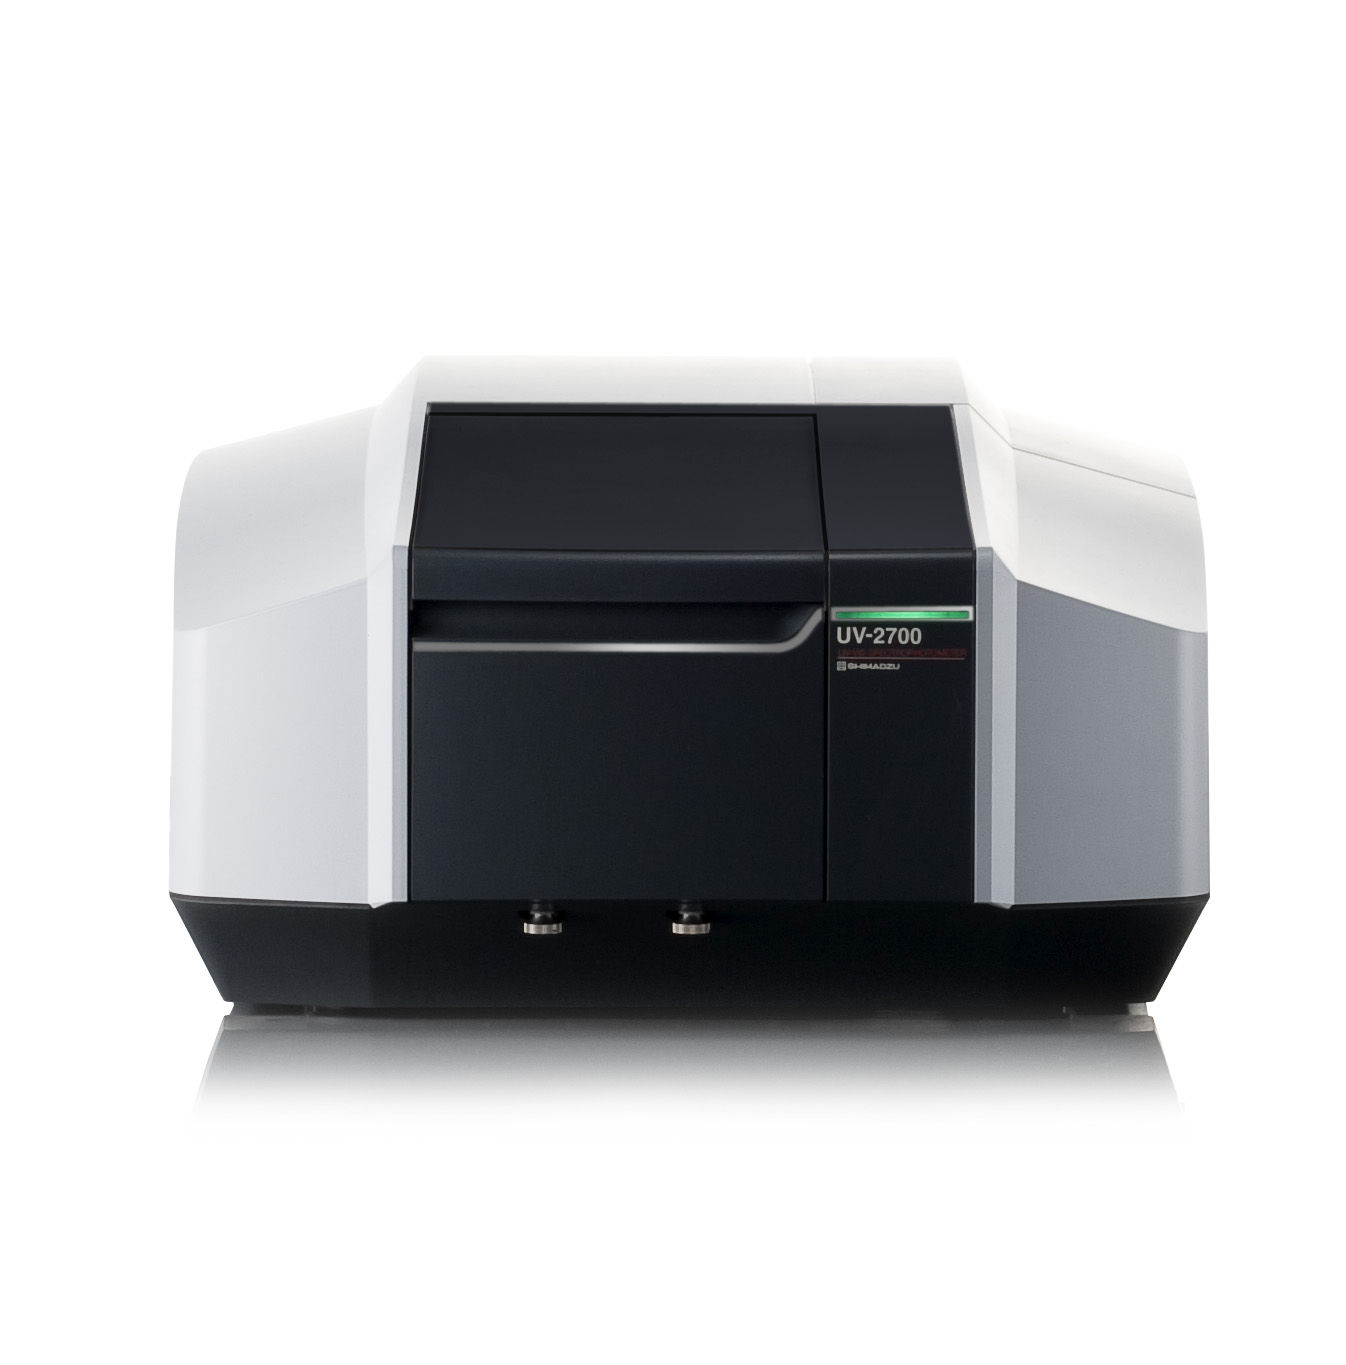
\includegraphics[width=\textwidth]{sources/uvviseq}
			\end{figure}
			\tiny
			\begin{itemize}
				\item Celdas de cuarzo.
				\item S = \ce{CH3CN} : \ce{H2O}
				\item C = 0.02 mM.
				\item 200 - 800 nm.
			\end{itemize}
		\end{column}
		\begin{column}{0.25\linewidth}
			\textbf{Fotoluminiscencia}
			\begin{figure}[h]
				\centering
				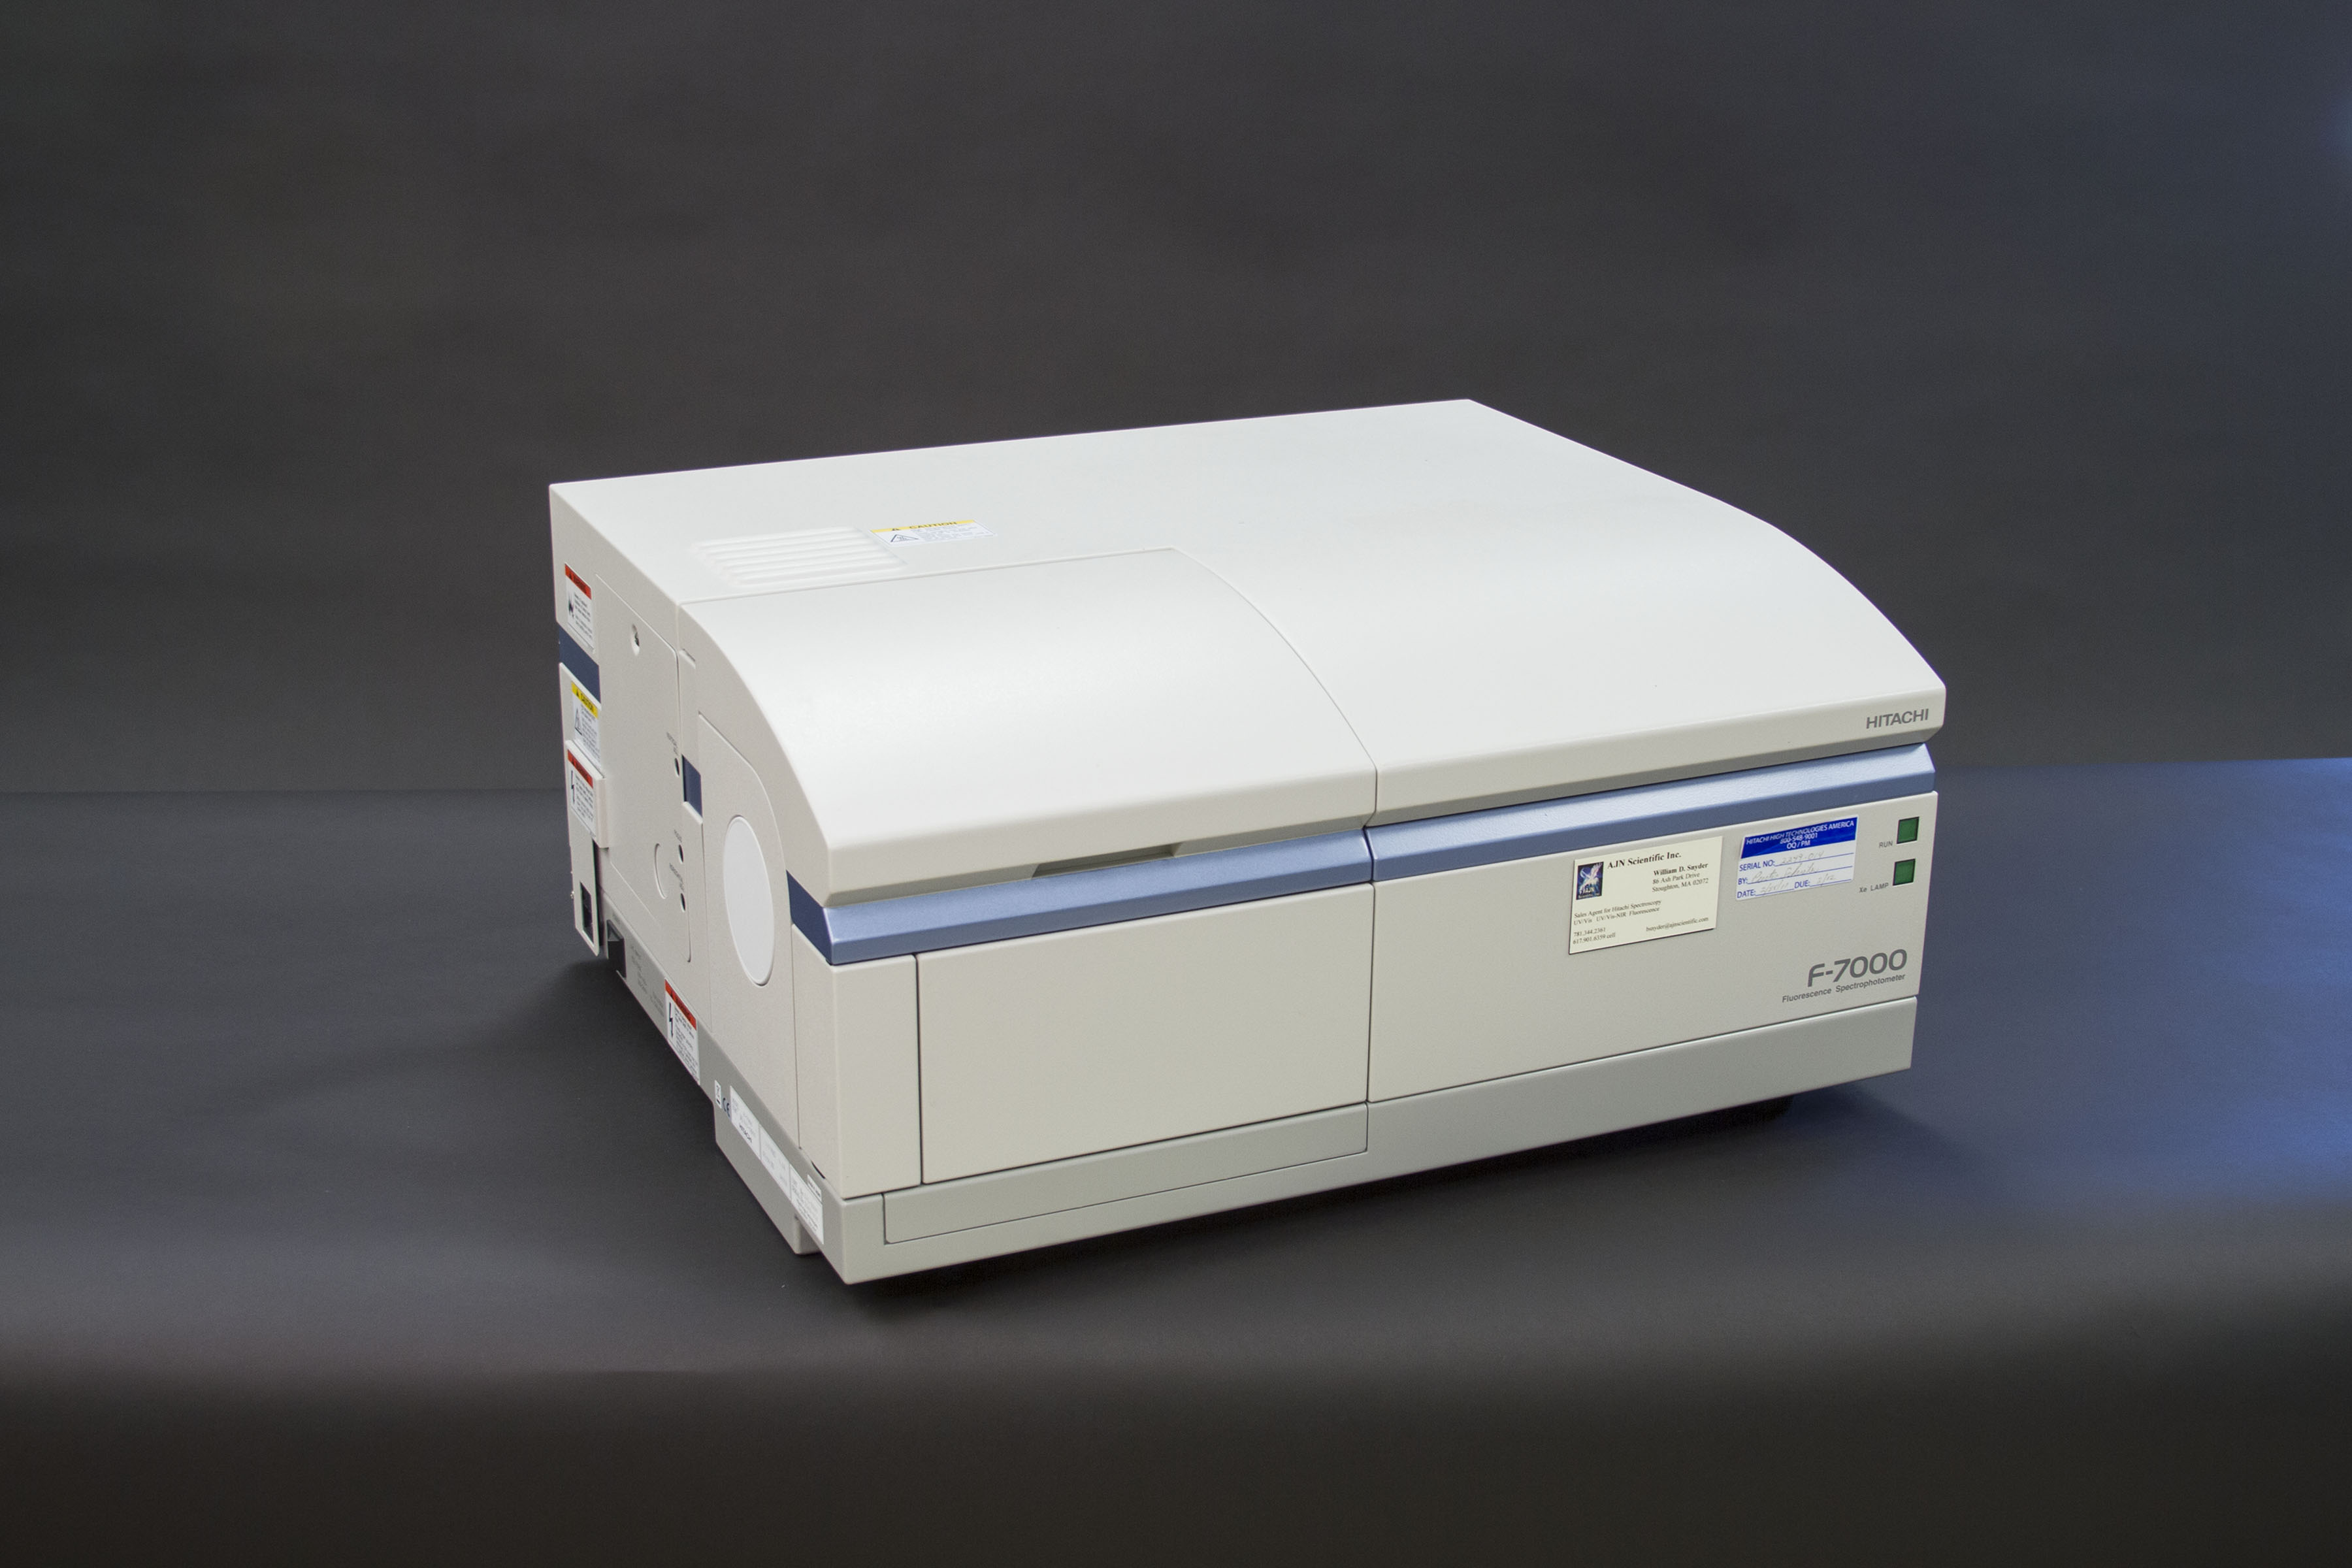
\includegraphics[width=\textwidth]{sources/fluorescence}
			\end{figure}
			\tiny
			\begin{itemize}
				\item Celdas de cuarzo.
				\item S = \ce{CH3CN} : \ce{H2O}
				\item C = 0.02 mM.
				\item 500 - 800 nm.
			\end{itemize}
		\end{column}
		\begin{column}{0.2\linewidth}
			\textbf{Electroqu\'imica}
			\begin{figure}[h]
				\centering
				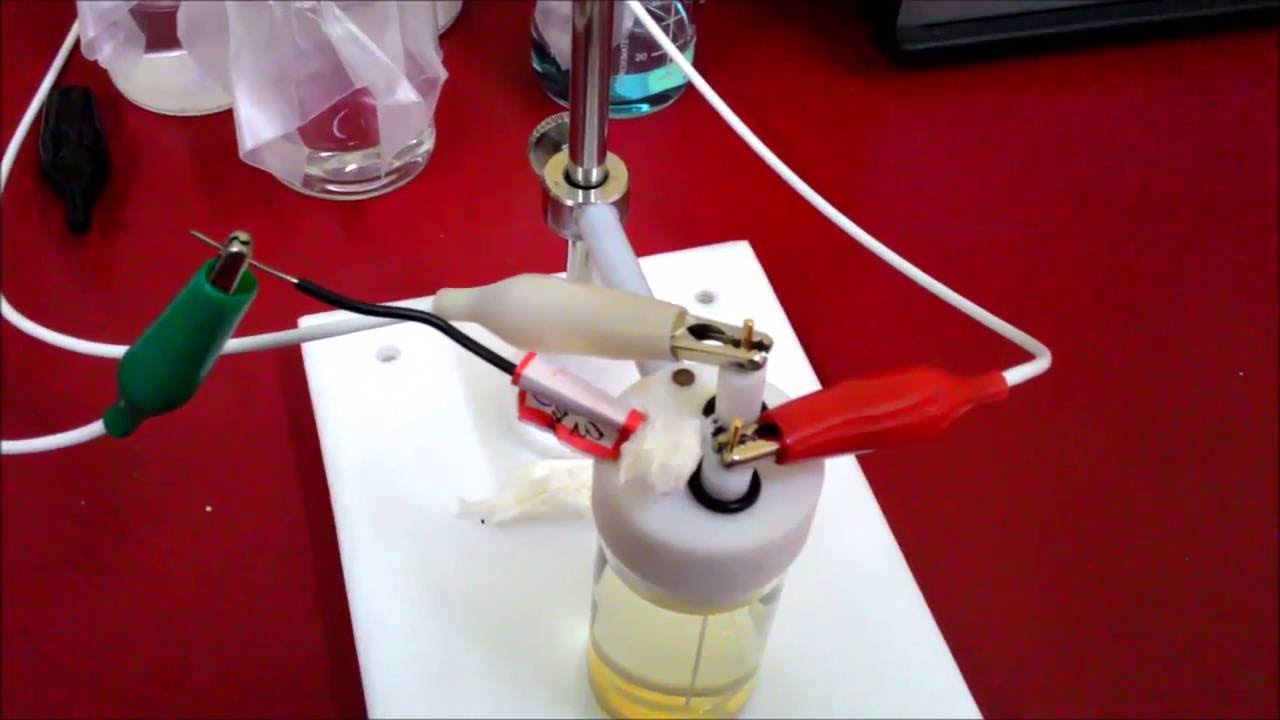
\includegraphics[width=\textwidth]{sources/electrical}
			\end{figure}
			\tiny
			\begin{itemize}
				\item WE: Pt
				\item RE: Ag/AgCl en KCl
				\item CE: Pt
			\end{itemize}
		\end{column}
	\end{columns}
	\vspace{1cm}
	KCl y \ce{(CH3CH2CH2CH2)4N(PF6)} son usados como electrolitos. Las soluciones son burbujeadas con \ce{N2} y \ce{CO2} por 40 minutos.
\end{frame}


\section{Resultados y discusi\'on}
\begin{frame}{Resultados y discusi\'on}
\end{frame}

\section{Conclusiones}
\begin{frame}{Conclusiones}
\end{frame}

\end{document}